\section{ХОД РАБОТЫ}

\subsection{Текст задания}

Необходимо написать два скрипта: первый скрипт должен установливать
программное обеспечение на компьютер с OC Windows, второй --- удалять
выбранные пользователем программы.

\subsection{Детали реализации скриптов}

В качестве программы для установки на компьютер выберем Python 2.7,
так как данная программа имеет установщик msi с возможностью
тихого и пассивного режимов установки.

Для начала проверим, установлен Python 2.7 на компьютере, или нет. Если
программа уже была установлена, то выводим сообщение и завершаем процесс
установки, в обратном случае --- начинаем процесс установки. Код, выполняющий
данные операции представлен на рисунке~\ref{lst:install_python}.

\begin{lstlisting}[caption=Проверка на существование Python 2.7 в системе,
label=lst:install_python,basicstyle=\scriptsize\ttfamily]
  $python = Get-WmiObject Win32_product | where-object {$_.Name -Like "Python*"}

  if ($python) {
      Write-Host "Python is already installed on your host! Skip installation"
  } else {
      Write-Host "Installing python 2.7..."
      ...
  }
\end{lstlisting}

Далее следует выбрать правильный установщик для Python. Для этого нужно
определить битность системы. Функция, определяющая битность системы
приведена на рисунке~\ref{lst:get_arch}.

\begin{lstlisting}[caption=Определение битности системы,
label=lst:get_arch,basicstyle=\scriptsize\ttfamily]
  Function Get-OS_Arch() {
      $arch = $(Get-WmiObject Win32_OperatingSystem).OSArchitecture

      if ($arch -Like "*64*")     { $arch = 64 }
      elseif ($arch -Like "*32*") { $arch = 32 }

      $arch
  }
\end{lstlisting}

Зная битность системы, можем начать установку программы. В случае 32-битной
системы, установка будет выполняться следующей командой:

\textit{.\textbackslash msi\textbackslash python-2.7.6.msi /passive}

Исходный текст разработанного скрипта расположен в приложении~А.



Для написания скрипта удаления программ Windows создадим файл
с расширением .wsf (Windows Script File). Пример содержимого файла с расширением
.wsf представлен на рисунке~\ref{lst:wsf}.

\begin{lstlisting}[caption=Пример содержимого файла с расширением .wsf,
label=lst:wsf,basicstyle=\scriptsize\ttfamily,language=VBScript]
 <job>
   <script language = "VBScript">
     ...
     ' script on VBScript language
     ...
   </script>
 </job>
\end{lstlisting}

С помощью WMI получим список всех установленных приложений. Представим это список
пользователю для выбора программы для удаления. В случае выбора программы для
удаления, пользователю останется лишь подтвердить правильность своего выбора.
После подтверждения процесс удаления программы будет запущен.

Скрипт получения списка установленных программ в OC Windows, написанный
на VBScript приведен на рисунке~\ref{lst:processes}.

\begin{lstlisting}[caption=Скрипт получения списка установленных программ \\
на языке VBScript,
label=lst:processes,basicstyle=\scriptsize\ttfamily,language=VBScript]
 Set objWMIService = GetObject("winmgmts:\\" & strComputer & "\root\cimv2")
 Set cProducts = objWMIService.ExecQuery("SELECT Name FROM Win32_Product")
\end{lstlisting}

Скрипт удаления программы представлен на рисунке~\ref{lst:delete_program}.
Параметр choice в данном скрипте --- порядковый номер установленной программы в
списке, предоставленном пользователю.

\begin{lstlisting}[caption=Скрипт удаления выбранной пользователем программы,
label=lst:delete_program,basicstyle=\scriptsize\ttfamily,language=VBScript]
 query = "SELECT * FROM Win32_Product WHERE Name ='" & productsArr(choice) & "'"
 Set cProducts = objWMIService.ExecQuery(query)
 For Each product in cProducts
   product.Uninstall()
 Next
\end{lstlisting}

Процесс исполнения скрипта \textit{delete\_program.wsf} приведен на
рисунках~\ref{fig:process} и~\ref{fig:delete_confirmation}.

\begin{figure}[htbp]
  \centering
  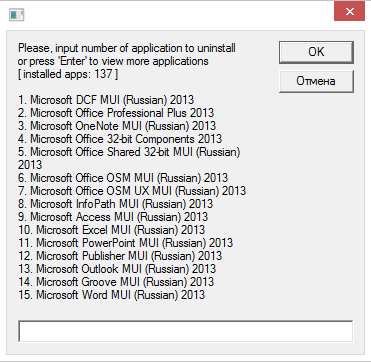
\includegraphics[width=110mm,height=100mm]{img/process}
  \caption{Процесс исполнения скрипта: вывод списка \\
   установленных в системе программ}
  \label{fig:process}
\end{figure}

\begin{figure}[htbp]
  \centering
  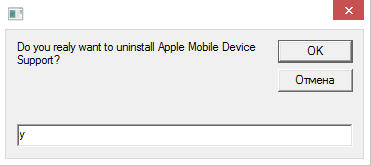
\includegraphics[width=100mm,height=45mm]{img/delete_confirmation}
  \caption{Подтверждение удаления программы}
  \label{fig:delete_confirmation}
\end{figure}

Исходный текст разработанного скрипта расположен в приложении~Б.

\newpage
